\documentclass[11pt, oneside]{article}   	%standardeinstellung
\usepackage{amsmath}				%damit du formeln eingeben kannst
\usepackage[parfill]{parskip}    			% neuer absatz durch leere zeile
\usepackage{graphicx}				% bilder einfügen
\usepackage[onehalfspacing]{setspace}	%1,5 facher zeilenabstand
\usepackage{hyperref}				%damit man links erstellen kann
\usepackage{float}					%intelligentes anpassen von bildern, damit es keine lücken im text gibt
\graphicspath{ {figures/} }				%automatisches erstellen von "List of Figures"
\usepackage[font=small,labelfont=bf]{caption} %formatierung der bildunterschrift
 \usepackage{geometry}				%Seitenlayout
 \usepackage{tikz}
 \usetikzlibrary{shapes,arrows}

 \geometry{						%musst du nicht unbedingt selbst einstellen
 a4paper,
 total={210mm,297mm},
 left=15mm,
 right=15mm,
 top=25mm,
 bottom=20mm,
 }

\usepackage{amssymb}
\usepackage{caption}
\usepackage{natbib}
\usepackage[utf8]{inputenc}
\usepackage{amsmath}
\usepackage{amsfonts}
\usepackage{amssymb}
\usepackage{wrapfig}
\usepackage{subcaption}
\usepackage{pdflscape}
\usepackage{soul}
\usepackage[space]{grffile}

\def\checkmark{\tikz\fill[scale=0.4](0,.35) -- (.25,0) -- (1,.7) -- (.25,.15) -- cycle;}

\title{Progress Report for MPhil Thesis}
\author{Tilman Graff -- University of Oxford}
\date{\today}

\begin{document}

\tikzstyle{data} = [draw, ellipse, fill=blue!20,
    text width=4.5em, text centered, node distance=3cm, minimum height=4em]
\tikzstyle{input} = [draw, ellipse, fill=red!20,
    text width=4.5em, text centered, node distance=3cm, minimum height=4em]
\tikzstyle{output} = [draw, ellipse, fill=green!20,
    text width=4.5em, text centered, node distance=3cm, minimum height=4em]
\tikzstyle{program} = [rectangle, draw, fill=white!20,
    text width=5em, text centered, rounded corners, minimum height=4em]
\tikzstyle{line} = [draw, -latex']

\bibliographystyle{cantoni_copy}
\maketitle

\section*{Open Questions -- What I need to discuss}
Topics to be raised in my next supervisor meeting.

Below starts my latest progress report.

\noindent\rule{\textwidth}{0.4pt}

\section{Research Question}
\textbf{Which factors influence the global distribution of trade network optimality?}

In this thesis, I aim to create a (potentially) global -- in any case African -- dataset of trade network efficiency. Taking the spatial distribution of current economic activity and population as given, I use a model from a recent working paper to determine the optimal trade network for each country. I then compare each country's current road network to its optimal one and derive a measure of how far a country is currently away from its ideal self.

In a second step, I will then investigate the origins of this global distribution. Which factors led to the heterogeneities among countries today? Specifically, I will look at:

\begin{itemize}
  \item Do networks with large colonial infrastructure investments do better or worse today?
  \item Does tribal favoritism explain why some areas are lacking lucrative investment?
\end{itemize}

Ferdinand notes that the better these questions are, the more I will be scrutinised for the methodology. But that's what I want!

\section{Research steps}

In order to conduct this research, I will need to follow a series of steps and transfer data between multiple programming softwares. Here is a step-by-step guide, with progress as of \today:



\begin{itemize}
  \item[\checkmark] Find global raster data on population, night-lights, ruggedness, and colonial infrastructure investments.
  \item[\checkmark] Grid the world on 50x50km squares and aggregate finer-resolution data into those grids.
  \item \st{Locate the maximum population point within each grid and call this the (population) centroid of the grid.} I decided against this additional step. Mostly because I cannot figure out how to do it in QGIS. (And it's probably not that important?). Instead, I investigate travel times and distances between unweighted geometric centroids.
  \item[\checkmark] Use OpenStreetMap to find distance and average speed between neighboring gridcells.
  \item Use distance and ruggedness to calculate Infrastructure Building Cost Matrix $\delta^{I}_{i,k}$ for every country.
  \item Use average speed to calculate current Infrastructure Matrix $I_{i,k}$ for every country.
  \item Use distance to calculate (iceberg) Trade Constant Matrix $\delta^{\tau}_{i,k}$ for every country.
  \item Use $\delta^{I}_{i,k}$, $\delta^{\tau}_{i,k}$, and $I_{i,k}$ to find the optimal trade network $I^{*}_{i,k}$ and optimal tradeflows $Q^{*}_{i,k}$ for every country. This directly follows the \cite{fajgelbaum_optimal_2017} Working Paper. I know how to do this, I am however afraid that this might take too long.
  \item Compare $I_{i,k}$ and $I^{*}_{i,k}$ for every country to obtain a measure of network optimality $\zeta_{c}$ for every country $c$.
  \item Investigate heterogeneity in $\zeta_{c}$

\end{itemize}

The following flowchart visualises the process. It shows the path input data (red circles) take through various programming languages (white rectangles) and intermediate datasets (blue circles) into eventual findings (green circle).



\section{Notes on individual steps}

In this section, I provide a more detailed account of what I did in each of the above-mentioned steps.

\resizebox{1\textwidth}{!}{
\begin{centering}
\begin{tikzpicture}[node distance = 3cm, auto]
  \node [input] (Lights) {Night Lights};
  \node [input, below of=Lights] (Rugg) {Ruggedness};
  \node [input, above of=Lights] (Population) {Population};
  \node [program, right of=Lights] (QGIS) {QGIS};
  \node [data, right of=QGIS] (Centroids) {Grid Centroids};
  \node [program, right of=Centroids] (R) {R};
  \node [input, below of=Centroids] (Roads) {Road Network};
  \node [data, right of=R] (Infrastructure) {Infrastr. Matrix};
  \node [data, above of=Infrastructure] (Trade) {Trade Cost};
  \node [data, below of=Infrastructure] (Building) {Building Cost};
  \node [program, right of=Infrastructure] (Matlab) {Matlab};
  \node [data, right of=Matlab] (Opt) {Optimal Network};
  \node [program, below of=Building] (Stata) {Stata};
  \node [input, right of=Stata, node distance=4.5cm] (misc) {Expl. variables};
  \node [output, left of=Stata, node distance=4.5cm] (Findings) {Findings};

  \path [line] (Lights) -- (QGIS);
  \path [line] (Population) -- (QGIS);
  \path [line] (Rugg) -- (QGIS);
  \path [line] (QGIS) -- (Centroids);
  \path [line] (Centroids) -- (R);
  \path [line] (Roads) -- (R);
  \path [line] (R) -- (Infrastructure);
  \path [line] (R) -- (Trade);
  \path [line] (R) -- (Building);
  \path [line] (Building) -- (Matlab);
  \path [line] (Infrastructure) -- (Matlab);
  \path [line] (Trade) -- (Matlab);
  \path [line] (Matlab) -- (Opt);
  \path [line] (Opt) -- (Stata);
  \path [line] (Roads) -- (Stata);
  \path [line] (misc) -- (Stata);
  \path [line] (Stata) -- (Findings);

\end{tikzpicture}
\end{centering}
}


\subsection{Find global raster data}
I use two datasources to create a global raster dataset of relevant variables:
\begin{itemize}
\item Data on night lights, ruggedness, land suitability, altitude, malaria index, and precipitation comes from \cite{henderson_global_2018}. These are available on 25km x 25km grids. Most of the data are for the year 2010.
\item For census-level spatial population data, I use the Gridded Population of the World (GPW) database from the \cite{socioeconomic_data_and_applications_center_gridded_2016}. These are available on much finer resolution. This database is for the year 2015.
\end{itemize}

Using GIS, I aggregated these datasets to a 1-by-1 degree global grid (roughly 50km x 50km), following \cite{fajgelbaum_optimal_2017}. In doing so, I take spatial sums of lights and population, and spatial averages of ruggedness, malaria, and weather data.

\subsection{Construct Centroids}
For each of these gridcells, I calculate the geometric centroid. I do not weigh by population in constructing this centroid, as I have been unable to figure out how to do this. I will need to discuss whether this is ok.

I then crop all global centroids that are not over land. This leaves me with 59,059 gridcells. Doing this, I am aware that I will lose information: I cut gridcells that might be partially over land, as soon as their centroid is not over land. This approach will, however, create equidistant centroid locations, so I'm really just playing one disadvantage against the other.

I then attribute the centroids with the lights, population, and other data from the underlying gridcell. Thus, I act as if all people and all economic activity of a given cell were concentrated on the single centroid point. This is because \citeauthor{fajgelbaum_optimal_2017}'s model calculates trade between nodes, not areas. I find this to be a reasonable model simplification.

\subsection{Construct Global Road database}
I calculate the optimal route between any centroid and each of its eight surrounding neigbours. In doing so, I rely on the open source online project \textsc{Open Street Maps} (OSM), which is comparable to \textsc{Google Maps}, but allows for unlimited use of its API. I scrape OSM with an R-Package called \texttt{osrmRoute}. This package takes start and destination locations, sends them to OSM, and comes back with the optimal route, distance, and speed in virtually no time. I am amazed by how fast this is.

Two problems present itself:
\begin{enumerate}
  \item OSM's data supply is user generated and hence biased towards more prosperous areas. However, since I mostly care about big highways, I doubt there are all too glaring ommisions. Also, I care about relative inefficiencies within a country, not cross-section differences between countries.
  \item I tell OSM to find the optimal route for a car. However, in many remote areas, cars don't get you from A to B. \texttt{osrmRoute} then desparately tries to locate the user onto the nearest street (which could be far away!). I hence scrape the entire loc-by-loc route, and calculate the walking distance to the nearest street (and the walking distance from the end of the supplied route to the actual endpoint). I do so by taking direct paths and imply a walking speed of 4 km/h. I then calculate whether walking the entire distance from A to B is faster (not shorter, but faster!) than the route supplied by \texttt{osrmRoute}. If so, I replace the route with the walking route.
\end{enumerate}

\begin{figure}[h]
\centering
\caption{Road Networks for different countries as scraped off OSM}

\begin{subfigure}[c]{0.48\textwidth}
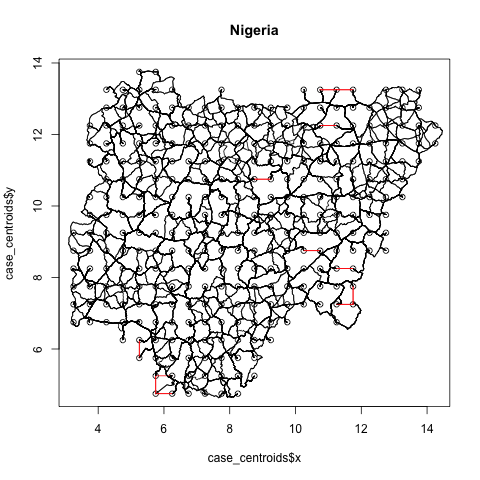
\includegraphics[width=\textwidth]{/Users/Tilmanski/Documents/UNI/MPhil/Second Year/Thesis_Git/Build/output/Road_Networks/network_Nigeria.png}
\caption{Nigeria}
\label{fig:nigeria}
\end{subfigure}
\begin{subfigure}[c]{0.48\textwidth}
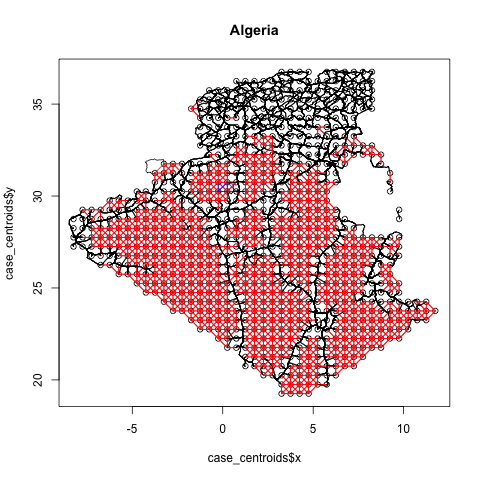
\includegraphics[width=\textwidth]{/Users/Tilmanski/Documents/UNI/MPhil/Second Year/Thesis_Git/Build/output/Road_Networks/network_Algeria.png}
\caption{Algeria}
\label{fig:algeria}
\end{subfigure}

\end{figure}

Figure \ref{fig:nigeria} displays how this would look like for the country of Nigeria. In black are optimal routes from all 289 centroids to their up to eight closest neighbours. If walking were the preferred option, this direct route is plotted in red. In Nigeria, this is mostly the case in some areas of the (swampy) South and East and some observations in the desert ridden North.

This procedure seems to well capture notions of remoteness: Consider the same graph but for Algeria (Figure \ref{fig:algeria}). For much of the Saharan parts of the country, walking straight lines through the sand is the best available option. I am actually not too worried about these areas. They will presumably have almost no population or night lights and hence I do not expect the later optimisation to yield unrealistic trans-Saharan highways.

\section{Calibration of $I_{i,k}$, $\delta^{\tau}_{i,k}$, $\delta^{I}_{i,k}$}

Next up, I use the obtained matrices to construct underlying graph characteristics needed for the model to work. As rough guideline, I follow \cite{fajgelbaum_optimal_2017}.

\subsection{Current Infrastructure Network $I_{i,k}$}
The matrix $I_{i,k}$ discretises the road network obtained by \texttt{osrmRoute}. Basically, it attaches a value to each link between nodes, indicating ``How much infrastructure'' has been built into the edge. \cite{fajgelbaum_optimal_2017} do this by calculating the mean number of lanes a road has plus adding a dummy for national roads. I cannot do this, as I don't have comprehensive data on road lanes. However, I believe that the derived speed matrix from \texttt{osrmRoute} actually serves as the much more significant statistic for what \citeauthor{fajgelbaum_optimal_2017} want to capture. I hence propose
\begin{equation}
  I_{i,k} = \textrm{Average Speed}_{i,k}
\end{equation}

\begin{figure}[!b]
  \centering
  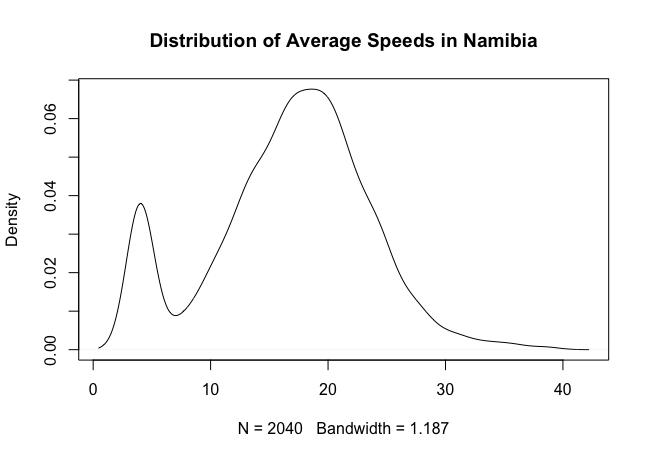
\includegraphics[width=0.7\textwidth]{/Users/Tilmanski/Documents/UNI/MPhil/Second Year/Thesis_Git/Build/output/Average Speeds/Speed_Namibia.png}
  \caption{Average Speed for Namibia, in km/h, 288 centroid locations}
  \label{fig:speed_namibia}
\end{figure}

This is obviously a very simple calibration and I am open to discuss more flexible approaches. But the general logic is clear: if a certain edge allows a car to drive faster on it, chances are that more investments had been made into it. In a sense, this captures the same notion \citeauthor{fajgelbaum_optimal_2017} with their calibration based on lanes and national roads. Figure \ref{fig:speed_namibia} shows a distribution of the average speeds (on travelled routes, in km/h) for Namibia. As can be seen, the distribution follows a nicely behaved shape, with an additional hump at 4 km/h for purely walked routes (see above).

\subsection{Infrastructure Building Cost Matrix $\delta^{I}_{i,k}$}

I am still working on this one. The entries to this matrix represent the cost to building new infrastructure (think: one additional km/h to stay in the logic from above) onto a given edge from $i$ to $k$. \citeauthor{fajgelbaum_optimal_2017} use

\begin{equation}
  \textrm{ln}(\frac{\delta^{I}_{i,k}}{dist_{i,k}}) = \textrm{ln}(\delta_{0}^{I}) - 0.11*(dist_{i,k} > 50km) + 0.12*\textrm{ln}(\textrm{ruggedness}_{i,k})
\end{equation}

which comes from \cite{collier_cost_2015}. $\delta_{0}^{I}$ is individual for every country. I have all the data to replicate this, but was thinking of including measures on extra low soil quality (which is congruent to Saharan soil) and (maybe) the Malaria index in there (or is that too much a colonial, \textit{``white guys walk in, build a road, and get Malaria''}, kind of thinking?)

\subsection{Iceberg Trade Constant Matrix $\delta^{\tau}_{i,k}$}

I follow \citeauthor{fajgelbaum_optimal_2017} in assuming

\begin{equation}
  \delta^{\tau}_{i,k} = \delta^{\tau}_{0} * dist_{i, k}^{\delta^{\tau}_{1}}
\end{equation}

where $\delta^{\tau}_{0}$ comes from a calibration using Spanish data and is reported -- and $\delta^{\tau}_{1} = 1$. I assume I can go ahead and use this replication.

The actual iceberg trade costs are then computed as

\begin{equation}
  \tau_{i,k}(Q_{i,k}, I_{i,k}) = \delta^{\tau}_{j, k} * \frac{Q_{i,k}^{\beta}}{I_{i,k}^{\gamma}}
\end{equation}

where $Q_{i,k}$ represents trade flows between nodes (to capture notion of congestion), $I_{i,k}$ is the existing Infrastructure Network (derived above), $\beta = 1$ and $\gamma = 1$ in the easiest calibration.

\section{Next steps}

\begin{enumerate}
  \item Decide on a stance regarding the questions raised above (1-2 days, possibly longer depending on how much to change)
  \item Calculate $I_{i,k}$, $\delta^{\tau}_{i,k}$, $\delta^{I}_{i,k}$ (2 hours)
  \item Optimise Matlab Code for better performance, or find better performance elsewhere (1 week)
  \item Perform Network optimisations (1-2 weeks)
\end{enumerate}

Immediate goal: Have optimal networks calculated by January 1, 2018.

\section*{Past supervisor meetings; topics raised and answered}

\subsection*{November 28, 2018}

\begin{itemize}
\item Is it ok to use geometric centroids as opposed to population-weighted centroids? \textit{Yes, it's fine. Ferdinand did this in \cite{maurer_mice_2017}.}
\item Night Lights: do I have to translate them into GDP first? \cite{fajgelbaum_optimal_2017} use G-Econ, but that's only available for the year 1990 and in much coarser resolution. \textit{Tough. But probably go for it just because it's easiest and no direct alternative comes to mind. Keep it at its easiest level. \cite{kocornik-mina_flooded_2015} do use pure lights and cite \cite{henderson_measuring_2012} who find a Lights-GDP elasticity of 1.}
\item Can I proceed to use Open Street Maps even though it has disadvantages as described below? \textit{Yes.}
\item Computational challenges looming. As soon as I'll start the Matlab bit, I will need either patience or better computing power. Does the department / chair grant access to remote desktops etc.? \textit{Probably not.}
\item Average speed a good proxy for Infrastructure Matrix $I_{i,k}$? \textit{Not really many other options.}
\item The paper by \cite{fajgelbaum_optimal_2017} has been criticised for its heavy dependence on the congestion assumption (in words, that iceberg trade costs rely on current tradeflows, or that $\tau_{i,k}(Q_{i,k}, I_{i,k})$ is a function of $Q_{i,k}$); namely by \cite{allen_welfare_2016}. I think this criticism is overblown. Still worth keeping in mind. \textit{Definitely cite and discuss this. But should be fine.}

\end{itemize}

\vspace{\fill}

\begin{spacing}{1.0}
\setlength{\bibsep}{2.5pt plus 1.5ex}
\bibliography{MPhil_library}
\end{spacing}

\end{document}
